\section{Problem No.2} \label{sec:prob2}
\subsection{Problem Description:} 
For solving the heat equation we frequently use \protect{\cn}, which is trapezoidal rule time integration with a second-order space discretization. The analogous scheme for the linear advection equation is 
$$
u_{j}^{n+1} - u_{j}^{n} + \frac{\nu}{4}(u_{j+1}^{n}-u_{j-1}^{n}) + \frac{\nu}{4}(u_{j+1}^{n+1}-u_{j-1}^{n+1}) =0,
$$
where $\nu = \frac{a\Delta t}{\Delta x}$
\begin{enumerate}
\item Use von Neumann analysis to show that this scheme is unconditionally stable and that $||u^{n}||_{2} = ||u^{0}||_{2}$. This scheme is said to be non-dissipative - i.e. there is no amplitude error. This seems reasonable because this is a property of the PDE.
\item Solve the advection equation on the periodic domain $[0,1]$ with the initial condition from problem 1 (part 2). Show the solution and comment on your results.
\item Compute the relative phase error as $\frac{arg(g(\theta))}{-\nu \theta}$, where $g$ is the amplification factor and $\theta=\zeta \Delta x$, and plot it for $\theta \in [0,\pi]$. How does the relative phase error and lack of amplitude error relate to the numerical solutions you observed in part 2. 
\end{enumerate}

\subsection{Solution:}
\paragraph{Part 1:}
To show that the scheme is unconditionally stable using von Neumann analysis, we start by assuming that the solution is of the form 
$$
u_{j}^{n}=e^{i\zeta x_{j}}\\
u_{j}^{n+1} = g(\zeta)e^{i\zeta x_{j}}
$$
where $g(\zeta)$ is the amplification factor and $\zeta$ is the wave number. In order to show the scheme is stable, $|g(\zeta)|\leq 1$. We start by plugging in the solution above in advection equation, the result will be 
$$
g(\zeta)e^{i\zeta x_{j}}-e^{i\zeta x_{j}} + \frac{\nu}{4}(e^{i\zeta (x_{j}+\Delta x)} - e^{i\zeta (x_{j}-\Delta x)})+ \frac{\nu}{4}(g(\zeta)e^{i\zeta (x_{j}+\Delta x)} - g(\zeta)e^{i\zeta (x_{j}-\Delta x)})=0
$$
Diving by $e^{i\zeta x_{j}}$ and arranging, the equation becomes
$$
g(\zeta)-1 + \frac{\nu}{4}(e^{i\zeta \Delta x} - e^{-i\zeta \Delta x})+ \frac{\nu}{4}(g(\zeta)e^{i\zeta \Delta x} - g(\zeta)e^{-i\zeta \Delta x})=0\\
g(\zeta) = \frac{1-\frac{\nu}{4}(e^{i\zeta \Delta x} -e^{-i\zeta \Delta x})}{1+\frac{\nu}{4}(e^{i\zeta \Delta x} -e^{-i\zeta \Delta x})}\\
g(\zeta) = \frac{1-i\frac{\nu}{2}sin(\zeta \Delta x)}{1+i\frac{\nu}{2}sin(\zeta \Delta x)}
$$
Taking the absolute value of the above
$$
|g(\zeta)|^{2} = \frac{1+ \frac{\nu^{2}}{4}sin^{2}(\zeta \Delta x)}{1+\frac{\nu^{2}}{4}sin^{2}(\zeta \Delta x)} = 1
$$
Since the $|g(\zeta)| \leq 1$, then the scheme is unconditionally stable. $\qquad \qquad \square$

To prove that $||u^{n}||_{2} = ||u^{0}||_{2}$, we start by arranging the advection equation so follows 
$$
u_{j}^{n+1}+\frac{\nu}{4}(u_{j+1}^{n+1}-u_{j-1}^{n+1}) = u_{j}^{n}-\frac{\nu}{4}(u_{j+1}^{n}-u_{j-1}^{n})
$$
Taking the sum squared of both sides
$$
\sum_{j}(u_{j}^{n+1}+\frac{\nu}{4}(u_{j+1}^{n+1}-u_{j-1}^{n+1}))^{2} = \sum_{j}(u_{j}^{n}-\frac{\nu}{4}(u_{j+1}^{n}-u_{j-1}^{n}))^{2}\\
\sum_{j}((u_{j}^{n+1})^{2}+\frac{\nu}{2}u_{j}^{n+1}(u_{j+1}^{n+1}-u_{j-1}^{n+1}) + \frac{\nu^{2}}{4}(u_{j+1}^{n+1}-u_{j-1}^{n+1})^{2}) =\\
\qquad \qquad \qquad \qquad \qquad \qquad \sum_{j}((u_{j}^{n})^{2}-\frac{\nu}{2}u_{j}^{n}(u_{j+1}^{n}-u_{j-1}^{n}) + \frac{\nu^{2}}{4}(u_{j+1}^{n}-u_{j-1}^{n})^{2})\\
\sum_{j}(u_{j}^{n+1})^{2} = \sum_{j}((u_{j}^{n})^{2} - \frac{\nu}{2}(u_{j}^{n}(u_{j+1}^{n}-u_{j-1}^{n}) + u_{j}^{n+1}(u_{j+1}^{n+1}-u_{j-1}^{n+1})) + \\
\qquad \qquad \qquad \qquad \qquad \qquad \qquad \qquad (\frac{\nu}{4})^{2}( (u_{j+1}^{n}-u_{j-1}^{n})^{2} - (u_{j+1}^{n+1}-u_{j-1}^{n+1})^{2} ))
$$

Since it's proven that $u_{j}^{n+1}=|g(\zeta)|u_{j}^{n}=u_{j}^{n}$, then 
$$
\sum_{j}(u_{j}^{n+1})^{2} = \sum_{j}((u_{j}^{n})^{2} - \frac{\nu}{2}(u_{j}^{n}(u_{j+1}^{n}-u_{j-1}^{n}) + u_{j}^{n}(u_{j+1}^{n}-u_{j-1}^{n})) + \\
\qquad \qquad \qquad \qquad \qquad \qquad \qquad \qquad (\frac{\nu}{4})^{2}( (u_{j+1}^{n}-u_{j-1}^{n})^{2} - (u_{j+1}^{n}-u_{j-1}^{n})^{2} ))\\
\sum_{j}(u_{j}^{n+1})^{2} = \sum_{j}((u_{j}^{n})^{2} - \nu u_{j}^{n}(u_{j+1}^{n}-u_{j-1}^{n}))\\
\sum_{j}(u_{j}^{n+1})^{2} = \sum_{j}((u_{j}^{n})^{2}) + \nu (\sum_{j} u_{j}^{n} u_{j-1}^{n} - \sum_{j} u_{j}^{n} u_{j+1}^{n})
$$

The product at grid point $j$ and the next point is the same as the product of $j$ and the previous point since it is a domain with periodic boundary conditions and we can imagine this as moving over a circle. 
$$
\sum_{j}(u_{j}^{n+1})^{2} = \sum_{j}((u_{j}^{n})^{2}) \\
||u^{n+1}||_{2} = ||u^{n}||_{2} 
$$
Thus, $||u^{n}||_{2} = ||u^{n-1}||_{2} =  ||u^{n-2}||_{2} ..... =  ||u^{0}||_{2} \qquad \qquad \qquad \square$ 
\newpage

\paragraph{Part 2:}
We can rewrite the equation as
$$
Au_{j}^{n+1} + Bu_{j+1}^{n+1} + Cu_{j-1}^{n+1} = D_{j}^{n}
$$
where
$$A=1, \;\; B=\frac{\nu}{4}, \;\; C=\frac{-\nu}{4}, \;\; D_{i}^{n}=u_{i}^{n}-\frac{\nu}{4}(u_{j+1}^{n}-u_{j-1}^{n})$$

The matrix formulation for the above equation for the periodic domain is 
\[
\left| \begin{array}{ccc ccccc}
A & B & 0 & 0 & ... & ... & 0 & C \\
C & A & B & 0 & ... & ... & 0 & 0 \\
0 & C & A & B & ... & ... & 0 & 0\\
... & ... & ... & ... & ... & ... & ... & ...\\
... & ... & ... & ... & ... & ... & ... & ...\\
... & ... & ... & ... & ... & ... & ... & ...\\
0 & 0 & ... & ... & 0 & C & A & B\\
B & 0 & ... & ... & 0 & 0 & C & A\\
\end{array} \right|
\left| \begin{array}{c}
u_{0}^{n+1} \\
u_{1}^{n+1} \\
u_{2}^{n+1} \\
...\\
...\\
...\\
u_{nx-2}^{n+1}\\
u_{nx-1}^{n+1}\\
\end{array} \right|
=
\left| \begin{array}{c}
D_{0}^{n} \\
D_{1}^{n} \\
D_{2}^{n} \\
...\\
...\\
...\\
D_{nx-2}^{n} \\
D_{nx-1}^{n} \\
\end{array} \right|
\]
The above system was solved using QR decomposition and the result is shown in Figure \ref{fig:cn} (b) for discontinuous initial conditions. It is clear that the scheme is not suitable for discontinuous initial conditions. 

\paragraph{Part 3:}
We start by deriving the expression $arg(g(\theta))$, where $\theta = \zeta \Delta x$ form the amplification factor such that
$$
g(\zeta) = \frac{1-i\frac{\nu}{2}sin(\zeta \Delta x)}{1+i\frac{\nu}{2}sin(\zeta \Delta x)}\\
g(\zeta) = \frac{1-\frac{\nu^{2}}{4}sin^{2}(\zeta \Delta x)}{1+\frac{\nu^{2}}{4}sin^{2}(\zeta \Delta x)} - i\frac{\nu sin(\zeta \Delta x)}{1+\frac{\nu^{2}}{4}sin^{2}(\zeta \Delta x)}\\
g(\zeta) = \frac{1-\frac{\nu^{2}}{4}sin^{2}(\theta)}{1+\frac{\nu^{2}}{4}sin^{2}(\theta)} - i\frac{\nu sin(\theta)}{1+\frac{\nu^{2}}{4}sin^{2}(\theta)}
$$
This gives the phase as
$$
arg(g(\theta)) = tan^{-1}(-\frac{\nu sin(\theta)}{1-\frac{\nu^{2}}{4}sin^{2}(\theta)})
$$
Figure \ref{fig:cn} (b) shows the relative phase error. The plot shows

\begin{figure}[!tbh]
 \centering        
   \subfloat [Solution]{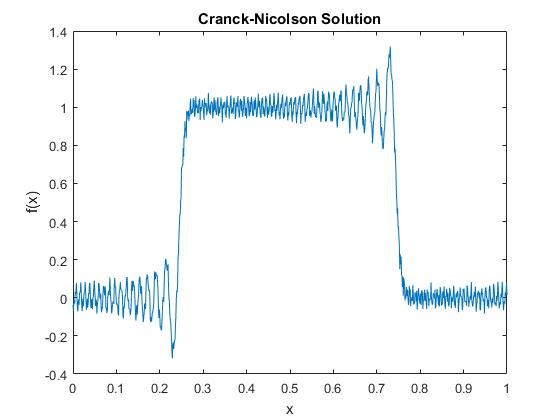
\includegraphics[width=0.5\textwidth]{fig/cn_nonsmooth.jpg}}
   \subfloat [Relative Phase]{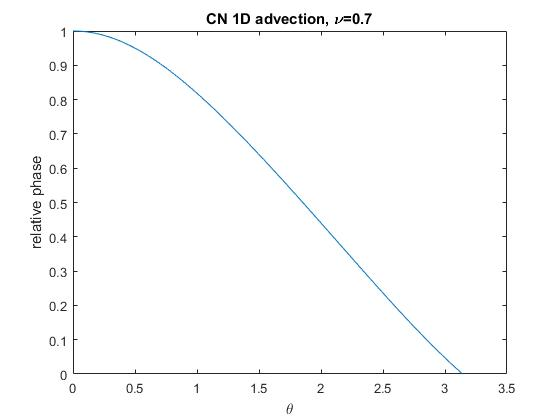
\includegraphics[width=0.5\textwidth]{fig/rev_phase.jpg}}
 
     \caption{Solution for of 1D advection equation using CN method; (a) shows the solution with discontinuous initial conditions and (b) shows the the relative phase error.}
   \label{fig:cn}
\end{figure} 